\section{Syllabus Unit Details}

%%%%%%%%%%%%%%%%%%%%%%%%%%%%%%%%%%%%%%%%%%%%%%%%%%%%%%%%%%%%%%%%%%%%%%%%%%%%%%%%%%%%%%%%%%%%%%%%%%%%%%%%%%%%%%%%%%%%%%%%
% Unit 1 : Quantum Foundations & Hardware
%%%%%%%%%%%%%%%%%%%%%%%%%%%%%%%%%%%%%%%%%%%%%%%%%%%%%%%%%%%%%%%%%%%%%%%%%%%%%%%%%%%%%%%%%%%%%%%%%%%%%%%%%%%%%%%%%%%%%%%%
\subsection*{Unit 1 - Quantum Foundations and Hardware}

%%%%%%%%%%%%%%%%%%%%%%%%%%%%%%%%%%%%%%%%%%%%%%%%%%%%%%%%%%%%%%%%%%%%%%%%%%%%%%%%%%%%%%%%%%%%%%%%%%%%%%%%%%%%%%%%%%%%%%%%
\subsubsection*{Introduction and Framing}\label{sec:U1-intro}
This opening unit situates quantum computing historically and conceptually.  
We contrast classical and quantum information, introduce qubits and elementary
gates, and survey the physical platforms that realise them.
The aim is to supply the shared vocabulary and intuition required for the more
formal mathematics and cryptographic material that follow.

%We present an introduction to the field of quantum computing. 
%We do this by setting out the historic origins and the fundamental concepts that distinguish it from classical computation.
%The unit introduces qubits and quantum gates, and looks briefly at the physical systems used to realise them.
%We aim to build in intuition and background to build the mathematical formalism introduced in subsequent units.

%A gentle introduction seeks to highlight why quantum computation is special.
%By understanding a little about how we create quantum particles and exotic quantum states, 
%the student should feel more confident in the more abstract concepts introduced as the unit progresses.

%Learners need a shared vocabulary (qubits, gates and physical realisations) before they can tackle algorithms or cryptographic threats. 
%A brief historical sketch and a tour of today's hardware ground the abstract mathematics that follows.

\begin{itemize}
	\item \textbf{Key message}: classical computers struggle to model quantum systems at scale; 
	quantum hardware was conceived to bridge that gap.
	\item Students encounter qubits, superposition, entanglement and the Bloch-sphere picture before any algorithmic detail.
\end{itemize}

%%%%%%%%%%%%%%%%%%%%%%%%%%%%%%%%%%%%%%%%%%%%%%%%%%%%%%%%%%%%%%%%%%%%%%%%%%%%%%%%%%%%%%%%%%%%%%%%%%%%%%%%%%%%%%%%%%%%%%%%
\subsubsection*{Intended Learning Outcomes}\label{sec:U1-LO}
By the end of Unit 1 each student will be able to
\begin{enumerate}[label=U1-\arabic*]
	\item explain Feynman’s simulation argument and its significance for quantum computation;
	\item represent an arbitrary single-qubit state in ket, column-vector and Bloch-sphere form, verifying normalisation;
	\item identify the major hardware platforms (superconducting, trapped-ion, photonic, annealing) 
	and discuss their practical trade-offs;
	\item describe an experimental set-up that manifests superposition or entanglement (e.\,g.\ polarised photons);
	\item execute a simple $H\!-\!\mathrm{CNOT}$ circuit on a cloud or local simulator and interpret the measurement histogram.
\end{enumerate}

%%%%%%%%%%%%%%%%%%%%%%%%%%%%%%%%%%%%%%%%%%%%%%%%%%%%%%%%%%%%%%%%%%%%%%%%%%%%%%%%%%%%%%%%%%%%%%%%%%%%%%%%%%%%%%%%%%%%%%%%
\subsubsection*{Indicative Reading}\label{sec:U1-reading}
\vspace{-0.4em}
\begin{enumerate}
	\item Feynman, R. (1986) \emph{\citetitle{Feynman:1986}}.
	\item Deutsch, D. (1985) \emph{\citetitle{Deutsch:1985}}.
	\item Preskill, J. (2023) \citetitle{Preskill:2023}.
	\item Nielsen, M. \& Chuang, I.\ (2010) \emph{\citetitle{Nielsen:2010}}, Chap.~1.
	\item Monroe, C.\ et al.\ (2021) \emph{\citetitle{Monroe:2021}}.
\end{enumerate}

%%%%%%%%%%%%%%%%%%%%%%%%%%%%%%%%%%%%%%%%%%%%%%%%%%%%%%%%%%%%%%%%%%%%%%%%%%%%%%%%%%%%%%%%%%%%%%%%%%%%%%%%%%%%%%%%%%%%%%%%
%\subsubsection*{Formative Assessments}\label{sec:U1-assessment}
%\begin{itemize}
%	\item Two low-stakes quizzes covering history and qubit representation.
%	\item Jupyter‐lab notebook: plot a random Bloch vector; run and	measure the Bell‐state circuit on IBM Qiskit simulator
%	(addresses U1-3 to U1-5).
%\end{itemize}


%%%%%%%%%%%%%%%%%%%%%%%%%%%%%%%%%%%%%%%%%%%%%%%%%%%%%%%%%%%%%%%%%%%%%%%%%%%%%%%%%%%%%%%%%%%%%%%%%%%%%%%%%%%%%%%%%%%%%%%%
\subsubsection*{Unit 1.1 - Quantum-Computing History}
Quantum computing originated with Feynman’s question \emph{"How do we simulate quantum physics?”} \cite{Feynman:1986} 
and was formalised by Deutsch’s universal quantum computer \cite{Deutsch:1985}.  
Preskill’s recent retrospective \cite{Preskill:2023} charts the path to modern NISQ devices.

\paragraph{In-class activity.}
Debate: "Why can’t a classical supercomputer simply simulate quantum systems?”  (aligns with outcome~U1-1).

%\emph{Purpose}: show that quantum computing arose from the practical question raised by Feynman, 
% "how do we simulate quantum physics?", 
% and evolved through Deutsch to modern NISQ devices.

%\emph{Key message}: classical computers struggle to model quantum systems; quantum hardware was conceived to close that gap.

%\emph{Outcomes}:
%\begin{itemize}
%	\item \emph{Explain} Feynman's simulation argument and its significance for quantum computation.
%\end{itemize}

%This unit draws on Preskill's paper \citetitle{Preskill:2023} \cite{Preskill:2023} (2023)
%and Feynman's \citetitle{Feynman:1986} (1986) \cite{Feynman:1986}, 
%to provide a historical context and initial motivation for quantum computing.

%Feynman introduces intuitively why quantum systems cannot be simulated efficiently by classical computers.
%He does this through the description of analogue simulation of physical quantum systems, 
%and so allows the student so see the contrast with digital quantum information processing with qubits and gates.
%A discussion on Deutsch's contributions - \citetitle{Deutsch:1985} \cite{Deutsch:1985} (1985) - offers context on this.


%%%%%%%%%%%%%%%%%%%%%%%%%%%%%%%%%%%%%%%%%%%%%%%%%%%%%%%%%%%%%%%%%%%%%%%%%%%%%%%%%%%%%%%%%%%%%%%%%%%%%%%%%%%%%%%%%%%%%%%%
\subsubsection*{Unit 1.2 - The Qubit: Representations and Realisations}

We model physical two-level systems (photon polarisation, electron spin, ion hyperfine states)
as basis vectors $\ket{0}$ and $\ket{1}$.

A general qubit is
\[
\ket{\psi} = \alpha\ket{0} + \beta\ket{1}, \qquad |\alpha|^{2}+|\beta|^{2}=1.
\]
Expressing 
$\alpha = \cos\frac{\theta}{2}$, $\beta = e^{i\phi}\sin\frac{\theta}{2}$ 
maps the state to a point on the Bloch sphere (Fig.~\ref{fig:bloch}).

\begin{figure}[ht] 
	\begin{adjustbox}{center}
		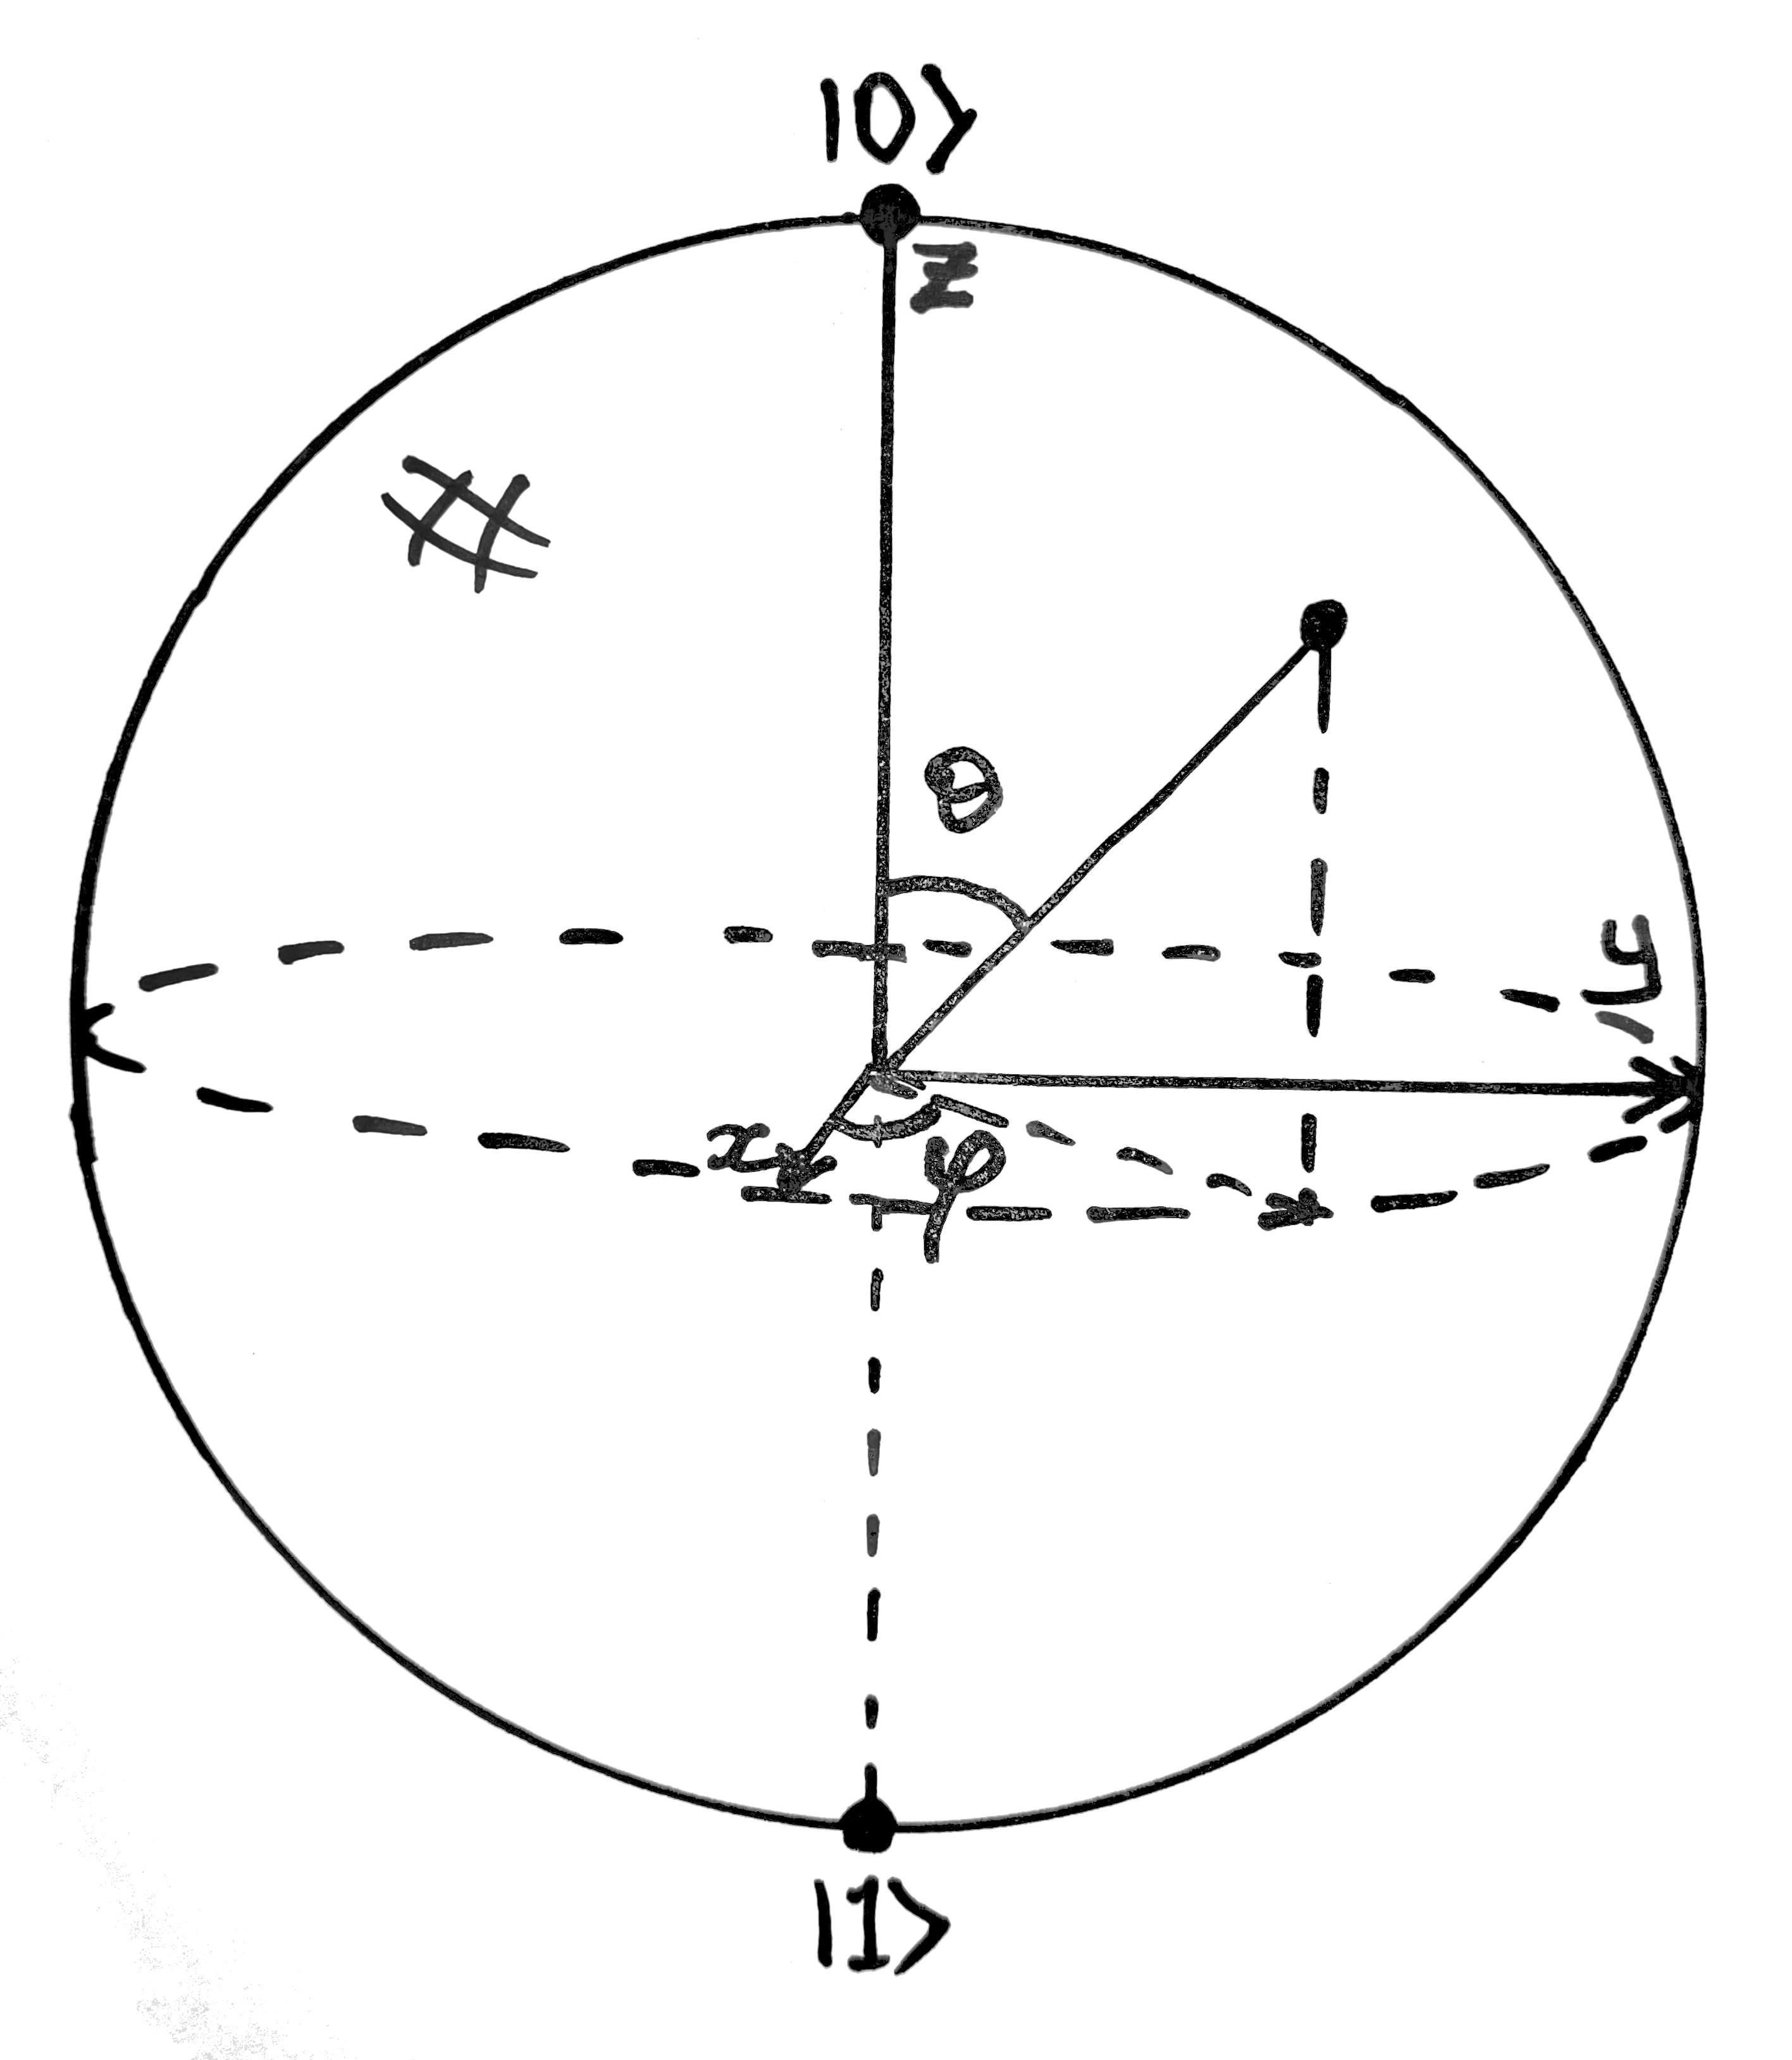
\includegraphics[width=0.3\textwidth, inner]{figures/blochsphere.png}
	\end{adjustbox}
	\vspace{4pt}
	\caption{Bloch sphere representation of a qubit}
	\label{fig:bloch}
\end{figure}


Superposition, the no-cloning theorem and entanglement are introduced
via single- and two-qubit examples.  Higher-level qudits (qutrits,
ququarts) are mentioned; their larger state spaces do \emph{not} yield
additional computational power \cite{Lipton:2021}.  

%\emph{Purpose}: define the qubit as a two-level quantum system and introduce the vector/Bloch-sphere picture.

%\emph{Key message}: superposition, no-cloning and entanglement distinguish qubits from bits, 
%yet all can be expressed in familiar linear-algebra terms. 
%Higher-level qudits exist but do not expand computational power beyond the qubit abstraction.

%\emph{Outcomes}:
%\begin{itemize}
%	\item \emph{Contrast} classical and quantum computing using the state-space (exponential) argument.
%\end{itemize}

%We introduced the qubit by talking about two-level quantum systems.
%Using examples of photons, trapped ions, quantum dots, superconducting quantum systems, 
%introduce the \emph{vector-state} representation and \emph{bloch-spheres}.
%Whilst talking about quantum states, we can introduce \emph{qudits}, such as \emph{qutrits} and \emph{quarts}.
%Drawing from $q$-ary linear code, we demonstrate the higher cardinality of three- and four-level quantum systems,
%and show that there is no loss in expressiveness in using the qubit abstraction.

%Introduce concepts of \emph{superposition}, \emph{no-cloning} and \emph{entanglement} in one and two qubit systems.
%Through this, introduce the \emph{Dirac} notation along side \emph{binary strings} and \emph{vector notation}
%as representations of superposition and entangled states.
%Use vector spaces and bloch spheres as a natural way of understanding a single qubit system.
%Measurement of computational basis states are discussed.

%We can use the introduction, and a high level, to demonstrate how quantum phenomenon can be manifested through physical systems.
%This can be as simple as using a set of polarising filters to see the ?? paradox.  
%The setup for photons to describe entanglement is straight forward, 
%but we can describe technique for ions and highlight how experimental physics is moving the industry forward 
%by reading \href{http://scienceblogs.com/principles/2009/07/07/entanglement-by-accident/}{Monroe on accidental ion entanglement}.

%%%%%%%%%%%%%%%%%%%%%%%%%%%%%%%%%%%%%%%%%%%%%%%%%%%%%%%%%%%%%%%%%%%%%%%%%%%%%%%%%%%%%%%%%%%%%%%%%%%%%%%%%%%%%%%%%%%%%%%%
\subsubsection*{Unit 1.3 - Quantum Machinery}
\paragraph{Hardware landscape.}
\begin{itemize}
	\item \emph{Analogue simulators}: cold atoms, Rydberg arrays (excel at condensed-matter models).
	\item \emph{Annealers}: D-Wave systems; tailored to Ising/QUBO optimisation.
	\item \emph{Photonic processors}: PsiQuantum, ORCA - natural fit for communication and QKD%
	\cite{ORCA:2022}\textbf{[citation needed for "earliest practical technology” and cost claim]}.
	\item \emph{Gate-based NISQ devices}: superconducting (IBM, Google), trapped-ion (IonQ, Honeywell); general-purpose algorithms.
\end{itemize}

Noise, decoherence and limited qubit counts motivate the distinction between NISQ and future fault-tolerant machines, 
foreshadowing quantum error-correction schemes.

%\emph{Purpose}: orient students within the hardware landscape; analogue simulators, annealers, photonic devices and gate-based processors.

%\emph{Key message}: different technologies excel in different niches 
%(e.g. photonics for communications, superconducting qubits for general algorithms), 
%and noise considerations motivate the distinction between NISQ and future fault-tolerant machines.

%\emph{Outcomes}:
%\begin{itemize}
%	\item \emph{Identify} the major hardware platforms and discuss their practical trade-offs.
%	\item \emph{Describe} at least one experimental set-up that manifests superposition or entanglement (e.g. polarised photons).
%\end{itemize}

%%%%%%%%%%%%%%%%%%%%%%%%%%%%%%%%%%%%%%%%%%%%%%%%%%%%%%%%%%%%%%%%%%%%%%%%%%%%%%%%%%%%%%%%%%%%%%%%%%%%%%%%%%%%%%%%%%%%%%%%
%%%%%%%%%%%%%%%%%%%%%%%%%%%%%%%%%%%%%%%%%%%%%%%%%%%%%%%%%%%%%%%%%%%%%%%%%%%%%%%%%%%%%%%%%%%%%%%%%%%%%%%%%%%%%%%%%%%%%%%%
% Unit 2 : Quantum Computation, Gates and Circuits (OBTL design)
%%%%%%%%%%%%%%%%%%%%%%%%%%%%%%%%%%%%%%%%%%%%%%%%%%%%%%%%%%%%%%%%%%%%%%%%%%%%%%%%%%%%%%%%%%%%%%%%%%%%%%%%%%%%%%%%%%%%%%%%
\subsection*{Unit 2 - Quantum Computation, Gates and Circuits}

This unit supplies the \emph{mathematical grammar} of quantum computing.  
Students translate the physical intuition gained in Unit 1 into linear-algebra formalism, postulates, 
universal gates and the circuit model, thereby laying a precise scaffold for every subsequent algorithmic idea.

\subsubsection*{Programme-level alignment}
\begin{itemize}
	\item \textbf{PL-1 Critical analysis}: prove and verify unitarity, reversibility, error-rates.
	\item \textbf{PL-2 Digital literacy}: implement and test circuits on Qiskit/Cirq simulators and hardware.
\end{itemize}

%%%%%%%%%%%%%%%%%%%%%%%%%%%%%%%%%%%%%%%%%%%%%%%%%%%%%%%%%%%%%%%%%%%%%%%%%%%%%%%%%%%%%%%%%%%%%%%%%%%%%%%%%%%%%%%%%%%%%%%%
\subsubsection*{Unit 2.1 - Linear Algebra \& State Representation}

\paragraph{Purpose}  
Provide the indispensable toolkit-vector spaces, inner products, matrix operators 
and tensor products-using the qubit as a running example.

%We start by recapping single- and dual-qubit vector states,  and give the generalization of \emph{quantum registers} used in quantum computing. 

\paragraph{Intended learning outcomes}
\begin{enumerate}[label=2.1-\arabic*]
	\item Express single- and multi-qubit states as column vectors and Dirac kets.
	\item Identify Hermitian, unitary and Pauli operators, 
	and explain why \emph{unitary} $\Longleftrightarrow$ \emph{reversible}.
	\item Compute simple tensor products and eigen-decompositions analytically and with \textsc{NumPy}.
	\item Depict a qubit in bra-ket, column-vector and Bloch-sphere co-ordinates.
\end{enumerate}

\paragraph{Key content}
\begin{itemize}
	\item Bases, linear independence and span.  
	\item Linear operators as matrices; inner products; eigenvalues and eigenvectors.  
	\item Pauli matrices; conjugate transpose (adjoint) and Hermitian operators.  
	\item Tensor products; commutators and anti-commutators.
%	\item Commutator and anti-commutator
	\item Polar and singular-value decompositions.
\end{itemize}

\vspace{0.5em}

%%%%%%%%%%%%%%%%%%%%%%%%%%%%%%%%%%%%%%%%%%%%%%%%%%%%%%%%%%%%%%%%%%%%%%%%%%%%%%%%%%%%%%%%%%%%%%%%%%%%%%%%%%%%%%%%%%%%%%%%
\subsubsection*{Unit 2.2 - Quantum Postulates}

\paragraph{Purpose}  
Anchor the algebra to the four standard postulates, emphasising Postulates 2 and 3 (dynamics) 
and Postulate 4 (composite systems).

\paragraph{Intended learning outcomes}
\begin{enumerate}[label=2.2-\arabic*]
	\item State each postulate in \emph{one sentence}.  
	\item Explain how unitary time-evolution (Post.~2) and projective measurement (Post.~3) coexist.  
	\item Give a concise explanation of why the Toffoli gate is the reversible \textsc{AND} analogue.  
	\item Illustrate each postulate with a direct two-line example.
\end{enumerate}

\begin{table}[h]
	\centering
	\begin{tabular}{p{0.24\linewidth}p{0.35\linewidth}p{0.33\linewidth}}
		\toprule
		\textbf{Postulate} & \textbf{Statement} & \textbf{Why it is dynamical} \\
		\midrule
		2. \emph{Unitary evolution} &
		$\ket{\psi(t)} = U(t,t_{0})\ket{\psi(t_{0})}$ with $U = e^{-iH(t-t_{0})/\hbar}$, $H = H^{\dagger}$ &
		Continuous, reversible law for amplitude flow (Schrödinger equation). \\[4pt]
		3. \emph{Projective measurement} & Measuring $M$ with projectors $\{P_{k}\}$ gives outcome
		$k$ with $p_{k}=\bra{\psi}P_{k}\ket{\psi}$ and post-measurement state $P_{k}\ket{\psi}/\sqrt{p_{k}}$ &
		Non-unitary update; explains definite outcomes. \\
		\bottomrule
	\end{tabular}
	\vspace{4pt}
	\caption{Postulates governing quantum dynamics.}
	\label{tab:postulates}
\end{table}

\paragraph{Classical vs quantum reversibility}
\begin{itemize}
	\item Truth table of classical \textsc{AND}: inputs cannot be recovered $\;\Rightarrow\;$ information loss.  
	\item Toffoli gate: adds a control qubit to make \textsc{AND} reversible and unitary.  
\end{itemize}

\paragraph{Block-encoding teaser}
Adding an ancilla qubit initialised to $\ket{0}$ allows us to embed a (non-unitary) matrix $A$ 
inside a larger unitary $U_{A}$; scaling factor $\alpha$ relates success probability.  
This idea underpins HHL, QSVT and quantum kernel algorithms.

\vspace{0.5em}


%\emph{Foundational Postulates}
%\begin{itemize}
%	\item \textbf{Postulate 1:} A quantum state is a vector in Hilbert space.
%	\item \textbf{Postulate 4:} Composite systems are described by the tensor product of individual system spaces.
%\end{itemize}
%
%These two postulates set the stage, but they do not directly govern dynamical evolution.
%
%\emph{Postulates Governing Dynamics}
%	\begin{table}[ht]
%		\centering
%		\renewcommand{\arraystretch}{0.2}
%		\begin{tabular}{|p{2.0cm}|p{4.0cm}|p{5.0cm}|p{4.0cm}|}
%			\textbf{\#} & \textbf{Postulate} & \textbf{What it says} & \textbf{Why it's "dynamics”} \\
%			\hline
%			\textbf{2. Unitary Time Evolution} & If a system is isolated during the interval $ t_0 \to t $, its state vector evolves by a \textbf{unitary} operator $ U(t,t_0) $. In the Schrödinger picture: & $ U(t,t_0) = \exp\!\bigl[-\,iH(t-t_0)/\hbar\bigr] $, where $ H $ is the system's Hermitian Hamiltonian. & This gives the reversible, deterministic law (Schrödinger equation) for how amplitudes flow, analogous to Newton's laws for classical trajectories. \\
%			\hline
%			\textbf{3. Measurement (Projective Version)} & Measuring an observable $ M $ with eigenvalues $ \{m_k\} $ and projectors $ \{P_k\} $ produces outcome $ m_k $ with probability $ p_k=\langle\psi|P_k|\psi\rangle $. After measurement, the system jumps to: & $ P_k|\psi\rangle/\sqrt{p_k} $. & This is the \textbf{non-unitary} dynamical rule that accounts for interaction with a detector and explains why we observe definite outcomes despite quantum interference. \\
%			\hline
%		\end{tabular}
%		\vspace{4pt}
%		\caption{Postulates governing dynamics in quantum mechanics}
%	\end{table}

%\emph{Summary}
%Postulate 2 provides the continuous, reversible evolution between measurements, while Postulate 3 supplies the stochastic, irreversible update during measurement. Together, they form the complete dynamical framework of standard quantum %theory.

%\emph{Qubit and unitarity rule}:
%\begin{itemize}
%	\item Define qubit $|psi\rangle = \alpha |0\rangle + \beta |1\rangle⟩$.
%\item State "Quantum mechanics says evolution is linear and norm-preserving $\Rightarrow$ matrices must be unitary."
%\end{itemize}

%\emph{Unitary $\iff$ reversible}:
%\begin{itemize}
%	\item Prove quickly: $U^\dag$ is both the inverse and the transpose-conjugate; multiplying restores the identity.
%\end{itemize}

%\emph{Circuit as factorisation}
%\begin{itemize}
%	\item Stack three 2×2 matrices; note the product is still unitary.
%	\item Draw the same gates in reverse order with daggers = inverse circuit.
%\end{itemize}

%\emph{Non-unitary aspirations}:
%\begin{itemize}
%	\item "We want to multiply by a real-valued data matrix or Hamiltonian; those aren't unitary!"
%\end{itemize}

%\emph{Block-encoding mechanics}:
%\begin{itemize}
%	\item Add one ancilla qubit initialised to $|0\rangle$.
%	\item Show that controlling on the ancilla embeds $A/\alpha$ in the top-left corner of the full matrix.
%	\item Stress the scaling factor αα and the success-probability interpretation.
%\end{itemize}

%\emph{Why:}
%\begin{itemize}
%	\item Mention HHL, QSVT, quantum kernels: "All call a block-encoding as a subroutine."
%	\item End with the mantra: "Circuits implement unitaries; block-encodings let those unitaries secretly carry the matrices we care about."
%\end{itemize}

%\emph{Why Irreversibility shows up in practice}
%\begin{enumerate}
%	\item Measurement - Projective measurement applies a non-unitary "collapse" operator. 
%	Information about the phase relations among amplitudes is discarded, so you cannot un-measure a generic outcome.

%	\item Open systems / decoherence - Coupling to an environment causes the joint evolution (system + bath) to stay unitary, 
%	but the reduced state of the system alone evolves under a completely-positive trace-preserving (CPTP) map, 
%	which is generally not invertible. 
%	Apparent irreversibility is just the price of ignoring the environment's qubits.
%\end{enumerate}

%\paragraph{Superdense Coding}:
%\begin{itemize}
%	\item Bell states and EPR
%\end{itemize}

%\paragraph{Density Operator}

%\paragraph{Schmidt decomposition and purifications}


%%%%%%%%%%%%%%%%%%%%%%%%%%%%%%%%%%%%%%%%%%%%%%%%%%%%%%%%%%%%%%%%%%%%%%%%%%%%%%%%%%%%%%%%%%%%%%%%%%%%%%%%%%%%%%%%%%%%%%%%
\subsubsection*{Unit 2.3 - Basic Gates \& Operations}

\paragraph{Purpose}  
Expound the universal gate set and develop the circuit picture.

\paragraph{Intended learning outcomes}
\begin{enumerate}[label=2.3-\arabic*]
	\item Build a three-gate circuit (e.g.\ $H$-CNOT-$Z$) and predict outcome probabilities.  
	\item Describe the no-cloning theorem and its impact on quantum communication.  
	\item Apply single- and two-qubit unitary gates and compute resulting state vectors.  
	\item Execute a simple circuit in Qiskit or Cirq and verify theory
	against simulator output.
\end{enumerate}

\paragraph{Concepts covered}
\begin{itemize}
	\item Bra-ket notation, column vectors in $\mathbb{C}^{2}$.  
%	\item Bra-ket notation and state representation; a way of writing vectors in a 2-D vector space: $|v \rangle \in \mathbb{C}^2$
%	\index{Bra-ket Notation}
	\item Matrix transformations of quantum states and gates
	\item Pauli ($X$, $Y$, $Z$), Hadamard ($H$), CNOT, phase shifts, controlled gates.  
	\item Reversibility $\; \Longleftrightarrow \;$ unitarity.  
	\item No-Cloning theorem: proofs and intuitive reasoning, consequences for quantum communication and cryptography.
\end{itemize}

\paragraph{Workshops}
\begin{itemize}
	\item \textbf{IBM Qiskit}: core gate library, interactive circuit composer.  
	\item \textbf{Google Cirq}: custom gate implementation and visualisers.
\end{itemize}

\vspace{0.5em}


%%%%%%%%%%%%%%%%%%%%%%%%%%%%%%%%%%%%%%%%%%%%%%%%%%%%%%%%%%%%%%%%%%%%%%%%%%%%%%%%%%%%%%%%%%%%%%%%%%%%%%%%%%%%%%%%%%%%%%%%
\subsubsection*{Unit 2.4 - Tensor Mathematics and Circuit Composition}

\paragraph{Purpose}  
Show how small gates scale to multi-qubit registers via tensor products and controlled operations.

\paragraph{Learning activities}
\begin{enumerate}[label=2.4-\arabic*]
	\item Rewrite a controlled-$U$ gate as a $2\times2$ block matrix.  
	\item Decompose a two-qubit gate into single-qubit rotations and CNOTs (lookup or SDK).  
	\item Assemble and run a short circuit on a cloud simulator; interpret the measurement statistics as a histogram.
\end{enumerate}

\paragraph{Suggested SDKs}
Qiskit Composer, Cirq tutorials, Julia~Yao.jl, Pennylane (automatic differentiation).

\vspace{0.5em}


%%%%%%%%%%%%%%%%%%%%%%%%%%%%%%%%%%%%%%%%%%%%%%%%%%%%%%%%%%%%%%%%%%%%%%%%%%%%%%%%%%%%%%%%%%%%%%%%%%%%%%%%%%%%%%%%%%%%%%%%
\subsubsection*{Unit 2.5 - NISQ Devices and Error-Correction Codes}

\paragraph{Purpose}  
Link the ideal circuit model to noisy hardware and introduce logical (encoded) qubits.

\paragraph{Intended learning outcomes}
\begin{enumerate}[label=2.5-\arabic*]
	\item Simulate a bit-flip error and show how a three-qubit repetition code detects it.  
	\item Distinguish NISQ error-mitigation from full fault tolerance.  
	\item Demonstrate a simple error-correction code protecting against a single-qubit error.  
	\item Discuss the trade-offs of on-chip state preparation versus hybrid	classical/quantum approaches.
\end{enumerate}

\paragraph{Key content}
Preskill’s NISQ overview; logical qubits; surface and colour codes (diagrammatic explanation); 
SDK demos of phase-flip and bit-flip correction.

\paragraph{Workshop tools}
\begin{itemize}
	\item Google Cirq (customizable noise models \& topological code simulations).
	\item IBM Qiskit Noise Simulator \& Ignis (specialized quantum error correction toolkit).
	\item \textsc{Stim}: Google's specialized quantum error correction simulator.
\end{itemize}

%%%%%%%%%%%%%%%%%%%%%%%%%%%%%%%%%%%%%%%%%%%%%%%%%%%%%%%%%%%%%%%%%%%%%%%%%%%%%%%%%%%%%%%%%%%%%%%%%%%%%%%%%%%%%%%%%%%%%%%%
%%%%%%%%%%%%%%%%%%%%%%%%%%%%%%%%%%%%%%%%%%%%%%%%%%%%%%%%%%%%%%%%%%%%%%%%
% Unit 3 : Quantum Algorithms and Classical Cryptography (OBTL design)
%%%%%%%%%%%%%%%%%%%%%%%%%%%%%%%%%%%%%%%%%%%%%%%%%%%%%%%%%%%%%%%%%%%%%%%%
\subsection*{Unit 3 - Quantum Algorithms and Classical Cryptography}

Students now discover \emph{why} quantum computing matters to security:
a small set of core algorithms (most famously Shor’s and Grover’s) break,
or seriously weaken, widely-deployed cryptographic protocols.  
The unit consolidates the linear-algebra skills from Unit\,2 
and introduces the algorithmic building-blocks required for Unit\,4.

%We then look at some subsequent algorithms that developed these ideas,
%building confidence with circuit complexity in preparation for more complex building blocks and algorithms in unit-4.

\subsubsection*{Over-arching outcomes}
By the end of Unit~3 each student will be able to
\begin{itemize}
	\item explain, at block-diagram level, how Shor’s and Grover’s algorithms threaten RSA, ECC and exhaustive search;
	\item build and run small instances of Deutsch-Jozsa, Simon, Grover and Shor circuits on a simulator, 
	interpreting the output;
	\item discuss the practical trade-offs between on-chip state preparation 
	and hybrid classical-quantum workflows on NISQ hardware.
\end{itemize}

%Use Shor's original paper as a motivating example for the ideas that were perfected subsequent to his paper:
%\begin{itemize}
%	\item Period finding as Quantum algorithm
%	\item Quantum phase estimation for modular multiplication and exponentiation 
%	\item Hidden Subgroup Problem in terms a eigenvalue (or phase) of a unitary operator
%	\item The unitary as an Oracle-like Component
%	\item Amplitude Amplification
%\end{itemize}


%%%%%%%%%%%%%%%%%%%%%%%%%%%%%%%%%%%%%%%%%%%%%%%%%%%%%%%%%%%%%%%%%%%%%%%%%%%%%%%%%%%%%%%%%%%%%%%%%%%%%%%%%%%%%%%%%%%%%%%%
\subsubsection*{Unit 3.1 - Classical Cryptography Problems}

\paragraph{Purpose}
Review the number-theoretic problems 
(integer factorisation, discrete logarithms, subset-sum) that underpin public-key and symmetric schemes, 
and outline the \emph{hidden-subgroup} formalism that generalises them.

\paragraph{Intended learning outcomes}
\begin{enumerate}[label=3.1-\alph*]
	\item State the mathematical statement of RSA factorisation and the discrete-log problem.                                     
	\item Map each problem to its hidden-subgroup instance.             
	\item Summarise in three sentences why a sub-exponential classical solution would endanger current protocols.                   
\end{enumerate}

%%%%%%%%%%%%%%%%%%%%%%%%%%%%%%%%%%%%%%%%%%%%%%%%%%%%%%%%%%%%%%%%%%%%%%%%%%%%%%%%%%%%%%%%%%%%%%%%%%%%%%%%%%%%%%%%%%%%%%%%
\subsubsection*{Unit 3.2 - Deutsch-Jozsa and Simon Algorithms}

\paragraph{Purpose}
Introduce the hidden-subgroup paradigm in its simplest forms; 
students practise reading small circuits and interpreting their algebraic output.

\paragraph{Intended learning outcomes}
\begin{enumerate}[label=3.2-\alph*]
	\item Build the Deutsch-Jozsa circuit for $n=3$ and predict the measurement string.                                          
	\item Show how Simon’s algorithm uses phase kick-back to reveal a hidden XOR mask.                                             
\end{enumerate}

%%%%%%%%%%%%%%%%%%%%%%%%%%%%%%%%%%%%%%%%%%%%%%%%%%%%%%%%%%%%%%%%%%%%%%%%%%%%%%%%%%%%%%%%%%%%%%%%%%%%%%%%%%%%%%%%%%%%%%%%
\subsubsection*{Unit 3.3 - Grover’s Algorithm}

\paragraph{Purpose}
Contrast amplitude-amplification’s quadratic speed-up with the exponential speed-ups of Shor-type algorithms; 
reinforce the role of oracles, reflections and NISQ noise.

\paragraph{Intended learning outcomes}
\begin{enumerate}[label=3.3-\alph*]
	\item Construct a Boolean oracle as a unitary and embed it in a Grover iteration.                                                   
	\item Execute the circuit on a noisy simulator and compare success probability with the ideal case.                             
	\item Explain the no-cloning constraint on oracle construction for database search.                                             
\end{enumerate}

\paragraph{Workshop platform}
\textbf{IBM Qiskit}: Grover composer; noisy back-end option.

%%%%%%%%%%%%%%%%%%%%%%%%%%%%%%%%%%%%%%%%%%%%%%%%%%%%%%%%%%%%%%%%%%%%%%%%%%%%%%%%%%%%%%%%%%%%%%%%%%%%%%%%%%%%%%%%%%%%%%%%
\subsubsection*{Unit 3.4 - Quantum Phase Estimation (QPE) \& Modular Arithmetic}

\paragraph{Purpose}
Show that QPE is the work-horse subroutine behind Shor and many later algorithms; 
modular multiplication supplies a concrete oracle.

\paragraph{Intended learning outcomes}
\begin{enumerate}[label=3.4-\alph*]
	\item Implement three-qubit QPE for an eigenphase $e^{2\pi i/8}$.  
	\item Explain the role of modular exponentiation in Shor’s order-finding.  
	\item Identify bottlenecks in state preparation for large moduli on NISQ hardware.                                               
\end{enumerate}

\paragraph{Workshop platforms}
Qiskit (QFT tutorials, modular-exponentiation circuit); Pennylane (Fourier basis notebooks).

%%%%%%%%%%%%%%%%%%%%%%%%%%%%%%%%%%%%%%%%%%%%%%%%%%%%%%%%%%%%%%%%%%%%%%%%%%%%%%%%%%%%%%%%%%%%%%%%%%%%%%%%%%%%%%%%%%%%%%%%
\subsubsection*{Unit 3.5 - Quantum Fourier Transform (QFT)}

\paragraph{Purpose}
Link the Fourier basis to period-finding; demonstrate a compact circuit that students can simulate.

\paragraph{Intended learning outcomes}
\begin{enumerate}[label=3.5-\alph*]
	\item Decompose the three-qubit QFT into a gate sequence no deeper than eight layers.                                           
	\item Demonstrate addition modulo $2^{n}$ using QFT arithmetic.    
\end{enumerate}

%%%%%%%%%%%%%%%%%%%%%%%%%%%%%%%%%%%%%%%%%%%%%%%%%%%%%%%%%%%%%%%%%%%%%%%%%%%%%%%%%%%%%%%%%%%%%%%%%%%%%%%%%%%%%%%%%%%%%%%%
\subsubsection*{Unit 3.6 - Putting it All Together - Shor’s Algorithm}

\paragraph{Purpose}
Assemble state preparation, modular arithmetic, QFT and amplitude amplification into the complete quantum attack on RSA.

\paragraph{Intended learning outcomes}
\begin{enumerate}[label=3.6-\alph*]
	\item Implement a small instance of Shor’s algorithm (mod 15) on a simulator; extract the period and factor 15.                  
	\item Interpret the measurement statistics and identify failure modes.                                                        
\end{enumerate}

\paragraph{Workshop platforms}
Qiskit (interactive Shor tutorials); Pennylane (modular-arithmetic circuits).

%%%%%%%%%%%%%%%%%%%%%%%%%%%%%%%%%%%%%%%%%%%%%%%%%%%%%%%%%%%%%%%%%%%%%%%%%%%%%%%%%%%%%%%%%%%%%%%%%%%%%%%%%%%%%%%%%%%%%%%%
\subsection*{Unit 4 - Advanced Quantum Algorithms}

Having mastered core algorithms, students now meet the techniques that dominate current research
(matrix inversion, polynomial singular-value transforms, quantum optimisation and hybrid workflows)
so they can read, reproduce and extend state-of-the-art results:

\subsubsection*{Unit 4.1 - Quantum Matrix Inversion (with HHL)}

\emph{Purpose}: show how a quantum computer can invert a sparse, well-conditioned matrix
exponentially faster than classical algorithms, subject to data-loading and read-out caveats.

The Harrow-Hassidim-Lloyd (HHL) \cite{Harrow:2009} \cite{Lipton:2021} algorithm is an important piece of work, 
designed to solve the Quantum Linear System Problem (QLSP). 
QLSP can be understood by considering the classical Linear System Problem (LPS) where we seek a vector $x$
to satisfy the set of linear equations $Ax = b$.  QLSP takes  a sparse, well-conditioned matrix  $A$ 
and vector $b$, encoded as quantum states, and produces a quantum state $\lvert x\rangle$ as a solution.  
Solving this problem requires a quantum matrix inversion, which HHL provides.

This algorithm, although seminal, leaves a number of challenges to overcome before the quantum speed-up of the 
matrix inversion can be taken advantage of.  The first is that recovering the full classical description of the 
vector $x$ from the quantum state can be computationally expensive and add significant overhead.

The second we raise is the problem of \emph{Quantum Random Access Memory} (QRAM) 
and practical issues in providing fast QRAM and loading large amounts of classical data.  
This subject comes up in another advanced technique, block encoding.

%%%%%%%%%%%%%%%%%%%%%%%%%%%%%%%%%%%%%%%%%%%%%%%%%%%%%%%%%%%%%%%%%%%%%%%%%%%%%%%%%%%%%%%%%%%%%%%%%%%%%%%%%%%%%%%%%%%%%%%%
\subsubsection*{Unit 4.2 - Block Encoding \& Quantum Singular-Value Transformation (QSVT)}

\paragraph{Purpose}: present block encoding as the universal trick for hiding non-unitary matrices inside unitaries, 
and QSVT as the "polynomial filter" that subsumes Grover, Hamiltonian simulation and HHL.

We take a high-level approach to QSVT as it is mathematically challenging to present, involving Chebyshev polynomials,
quantum signal processing and a good amount of linear-algebra bookkeeping.

The core idea \emph{Block-Encoding} (BE) is that, if you can hide a non-unitary matrix $A$ inside of a matrix 
This core technique of BE comes up a lot in modern quantum algorithms, and it should be presented.  
Building on the concepts from Grover's AA, QPE, and Hamiltonian simulation, we present the motivation 
and the pattern of the solution.  
Indeed, the analogy of the QSVT as a digital filter acting on frequency components, should bolster earlier work with phases.

\paragraph{Outcome}:
\begin{itemize}
	\item Understand QSVT as polynomial singular-value transformations via controlled phase sequences.
	\item Identify Grover and Hamiltonian simulation as special cases.
	\item Describe an \emph{unitary control register} as block-encoding \emph{plus} an ancilla qubit.
	\item Run a prepared QSVT circuit on a toy, low-degree, matrix and verify the singular values.
\end{itemize} 

%%%%%%%%%%%%%%%%%%%%%%%%%%%%%%%%%%%%%%%%%%%%%%%%%%%%%%%%%%%%%%%%%%%%%%%%%%%%%%%%%
\subsubsection*{Unit 4.3 - Quantum Annealing \& QUBO (D-Wave)}

We introduce Ising and Quantum Unconstrained Binary Optimization (QUBO) models for quantum annealing.  
Problems that are typically tackled with theses models are discussed, 
principally optimisation problems, Hamiltonians, and energy landscapes of quantum chemistry.

\begin{itemize}
	\item Demonstrates hardware tailored to Ising/optimization problems and contrasts analogue with gate-model approaches.
 	\item D-Wave Leap (Quantum annealing experiments, practical QUBO solutions)
\end{itemize}

%%%%%%%%%%%%%%%%%%%%%%%%%%%%%%%%%%%%%%%%%%%%%%%%%%%%%%%%%%%%%%%%%%%%%%%%%%%%%%%%%
\subsubsection*{Unit 4.4 - Gate-model Optimisation (QAOA / VQE)}

\paragraph{Purpose}: the current focus has shifted towards heuristic algorithms, inspired by classical principles and quantum phenomena, 
like the \emph{Quantum Approximate Optimization Algorithm} (QAOA) and \emph{Variational Quantum Eigensolver} (VQE).
These heuristic methods are designed for NISQ devices, and lack provable guarantees but hold promise for practical applications.

\begin{itemize}
	\item Shows how variational circuits tackle the same problems on NISQ gate-based devices.
\end{itemize}

\textbf{Workshop SDKs/Platforms}:
\begin{itemize}
	\item Pennylane (variational quantum algorithms for optimization)
	\item Google Cirq (QAOA tutorials)
\end{itemize}

%%%%%%%%%%%%%%%%%%%%%%%%%%%%%%%%%%%%%%%%%%%%%%%%%%%%%%%%%%%%%%%%%%%%%%%%%%%%%%%%%
\subsubsection*{Unit 4.5 - Quantum Algorithms for Graph Problems}

Concrete optimization tasks (Max-Cut, colouring) that map neatly to both annealing and QAOA.

\emph{}
\begin{itemize}
	\item Graph coloring
	\item max-cut
	\item shortest path problems
\end{itemize}

\textbf{Workshop SDKs/Platforms}:
\begin{itemize}
	\item Google Cirq (QAOA for MaxCut, detailed graph problems examples)
	\item D-Wave Leap (Ising models, graph optimization problems)
\end{itemize}


%%%%%%%%%%%%%%%%%%%%%%%%%%%%%%%%%%%%%%%%%%%%%%%%%%%%%%%%%%%%%%%%%%%%%%%%%%%%%%%%%
\subsubsection*{Unit 4.6 - QML: QSVM}

\paragraph{Outcomes}:
\begin{itemize}
	\item \emph{Implement} a simple quantum kernel OC-SVM on a cloud platform and benchmark against a classical baseline.
\end{itemize}

\paragraph{ML Primer}
\begin{itemize}
	\item Kernels
	\item SVM math
	\item Anomaly-detection metrics
\end{itemize}

\paragraph{Quantum Kernels \& Feature Maps}
\begin{itemize}
	\item Swap-test
	\item Fidelity estimation
	\item Expressivity vs noise
\end{itemize}

\paragraph{Quantum OC-SVM Workflow}
\begin{itemize}
	\item Data-encoding circuits
	\item Kernel-matrix build on hardware (QVM or real)
	\item Classical QP (CVXOPT / LIBSVM) for support vectors
	\item Hybrid inference loop; noise-mitigation hacks
\end{itemize}


\paragraph{Workshop SDKs/Platforms}
\begin{itemize}
	\item Pennylane (best QSVM wrappers)
	\item Julia QML for high-performance simulations
	\item Implement OC-SVM in Pennylane
	\item Test against classical scikit-learn
\end{itemize}


\subsubsection*{Unit 4.7 - QML:Variational Classifiers}

\paragraph{Workshop SDKs/Platforms}:
\begin{itemize}
	\item Pennylane (core QML package, variational circuits)
	\item Julia QML/Yao tutorials (high-performance QML simulations)
\end{itemize}

\subsubsection*{Unit 4.8 - QML:Quantum Neural Nets}
\begin{itemize}
	\item Pennylane (smooth classical-to-quantum transition tutorials, quantum neural nets)
\end{itemize}


%%%%%%%%%%%%%%%%%%%%%%%%%%%%%%%%%%%%%%%%%%%%%%%%%%%%%%%%%%%%%%%%%%%%%%%%%%%%%%%%%
\subsubsection*{Unit 4.9 - Hybrid Classical-Quantum Systems}

\paragraph{Purpose}: teach students to treat the QPU as a remote accelerator within 
a larger data pipeline, mirroring how real projects are executed in the NISQ era.

Unit treats a quantum device as a remote accelerator via hybid-jobs api.
Exercises reinforce core quantum ideas; state preparation, measurement statistics, error mitigation.

The analogy: similarly to GPU or ML cloud resources (PyTorch, AWS SageMaker) 
quantum processes are an external call from the Python code to accelerate 
an specific loop, while local processing handles the data wrangling, optimisation, logging, etc.

\begin{itemize}
	\item rationale behind the use of hybrid classical-quantum computing in the NISQ era
	\item Swap test; measurement statistics
	\item Error mitigation
	\item error budgets
	\item Parameter-shift rule; unitarity	
\end{itemize}


\paragraph{Topics}
\begin{itemize}
	\item Kernel estimation: OC-SVM kernel loop
	\item Variational Quantum Algorithms (VQAs) workflows: 
	Frame VQAs (like QAOA or VQE) as prime examples of the hybrid paradigm, 
	highlighting the classical optimisation loop and the quantum circuit execution/measurement step; 
	VQE or QAOA on Braket Hybrid Jobs; 
	\item Data pipeline walk through ETL-to-QPU pipeline
\end{itemize}

\paragraph{Outcomes}:
\begin{itemize}
	\item Architect a pipeline that ingests classical time-series, invokes a quantum kernel routine, and performs classical optimisation.
	\item Quantify shot noise and latency, choosing batch sizes and iteration counts that respect cloud-QPU quotas.
	\item Deploy a simple hybrid job on either AWS Braket or IBM
	\item Classic/Quantum performance 
	\item TensorFlow Quantum (Cirq-based, optional for broader ML integrations)
	\item Julia Quantum ML/QML.jl (efficient QML experiments, classical-quantum hybrid models)
	\item \emph{Architect} a hybrid workflow that balances shot cost, latency and classical compute.
\end{itemize}